%!TEX TS-program = xelatex
\documentclass[10pt,oneside]{article}
\usepackage[fontsize=9pt]{scrextend}

\usepackage[english]{babel}

\usepackage{amsmath,amssymb,amsfonts}
\usepackage[utf8]{inputenc}
\usepackage[T1]{fontenc}
\usepackage{stix2}
\usepackage[scaled]{helvet}
\usepackage[scaled]{inconsolata}

\usepackage{lastpage}

\usepackage{setspace}

\usepackage{ccicons}

\usepackage[hang,flushmargin]{footmisc}

\usepackage{geometry}

\setlength{\parindent}{0pt}
\setlength{\parskip}{6pt plus 2pt minus 1pt}

\usepackage{fancyhdr}
\renewcommand{\headrulewidth}{0pt}\providecommand{\tightlist}{%
  \setlength{\itemsep}{0pt}\setlength{\parskip}{0pt}}

\makeatletter
\newcounter{tableno}
\newenvironment{tablenos:no-prefix-table-caption}{
  \caption@ifcompatibility{}{
    \let\oldthetable\thetable
    \let\oldtheHtable\theHtable
    \renewcommand{\thetable}{tableno:\thetableno}
    \renewcommand{\theHtable}{tableno:\thetableno}
    \stepcounter{tableno}
    \captionsetup{labelformat=empty}
  }
}{
  \caption@ifcompatibility{}{
    \captionsetup{labelformat=default}
    \let\thetable\oldthetable
    \let\theHtable\oldtheHtable
    \addtocounter{table}{-1}
  }
}
\makeatother

\usepackage{array}
\newcommand{\PreserveBackslash}[1]{\let\temp=\\#1\let\\=\temp}
\let\PBS=\PreserveBackslash

\usepackage[breaklinks=true]{hyperref}
\hypersetup{colorlinks,%
citecolor=blue,%
filecolor=blue,%
linkcolor=blue,%
urlcolor=blue}
\usepackage{url}

\usepackage{caption}
\setcounter{secnumdepth}{0}
\usepackage{cleveref}

\usepackage{graphicx}
\makeatletter
\def\maxwidth{\ifdim\Gin@nat@width>\linewidth\linewidth
\else\Gin@nat@width\fi}
\makeatother
\let\Oldincludegraphics\includegraphics
\renewcommand{\includegraphics}[1]{\Oldincludegraphics[width=\maxwidth]{#1}}

\usepackage{longtable}
\usepackage{booktabs}

\usepackage{color}
\usepackage{fancyvrb}
\newcommand{\VerbBar}{|}
\newcommand{\VERB}{\Verb[commandchars=\\\{\}]}
\DefineVerbatimEnvironment{Highlighting}{Verbatim}{commandchars=\\\{\}}
% Add ',fontsize=\small' for more characters per line
\usepackage{framed}
\definecolor{shadecolor}{RGB}{248,248,248}
\newenvironment{Shaded}{\begin{snugshade}}{\end{snugshade}}
\newcommand{\KeywordTok}[1]{\textcolor[rgb]{0.13,0.29,0.53}{\textbf{#1}}}
\newcommand{\DataTypeTok}[1]{\textcolor[rgb]{0.13,0.29,0.53}{#1}}
\newcommand{\DecValTok}[1]{\textcolor[rgb]{0.00,0.00,0.81}{#1}}
\newcommand{\BaseNTok}[1]{\textcolor[rgb]{0.00,0.00,0.81}{#1}}
\newcommand{\FloatTok}[1]{\textcolor[rgb]{0.00,0.00,0.81}{#1}}
\newcommand{\ConstantTok}[1]{\textcolor[rgb]{0.00,0.00,0.00}{#1}}
\newcommand{\CharTok}[1]{\textcolor[rgb]{0.31,0.60,0.02}{#1}}
\newcommand{\SpecialCharTok}[1]{\textcolor[rgb]{0.00,0.00,0.00}{#1}}
\newcommand{\StringTok}[1]{\textcolor[rgb]{0.31,0.60,0.02}{#1}}
\newcommand{\VerbatimStringTok}[1]{\textcolor[rgb]{0.31,0.60,0.02}{#1}}
\newcommand{\SpecialStringTok}[1]{\textcolor[rgb]{0.31,0.60,0.02}{#1}}
\newcommand{\ImportTok}[1]{#1}
\newcommand{\CommentTok}[1]{\textcolor[rgb]{0.56,0.35,0.01}{\textit{#1}}}
\newcommand{\DocumentationTok}[1]{\textcolor[rgb]{0.56,0.35,0.01}{\textbf{\textit{#1}}}}
\newcommand{\AnnotationTok}[1]{\textcolor[rgb]{0.56,0.35,0.01}{\textbf{\textit{#1}}}}
\newcommand{\CommentVarTok}[1]{\textcolor[rgb]{0.56,0.35,0.01}{\textbf{\textit{#1}}}}
\newcommand{\OtherTok}[1]{\textcolor[rgb]{0.56,0.35,0.01}{#1}}
\newcommand{\FunctionTok}[1]{\textcolor[rgb]{0.00,0.00,0.00}{#1}}
\newcommand{\VariableTok}[1]{\textcolor[rgb]{0.00,0.00,0.00}{#1}}
\newcommand{\ControlFlowTok}[1]{\textcolor[rgb]{0.13,0.29,0.53}{\textbf{#1}}}
\newcommand{\OperatorTok}[1]{\textcolor[rgb]{0.81,0.36,0.00}{\textbf{#1}}}
\newcommand{\BuiltInTok}[1]{#1}
\newcommand{\ExtensionTok}[1]{#1}
\newcommand{\PreprocessorTok}[1]{\textcolor[rgb]{0.56,0.35,0.01}{\textit{#1}}}
\newcommand{\AttributeTok}[1]{\textcolor[rgb]{0.77,0.63,0.00}{#1}}
\newcommand{\RegionMarkerTok}[1]{#1}
\newcommand{\InformationTok}[1]{\textcolor[rgb]{0.56,0.35,0.01}{\textbf{\textit{#1}}}}
\newcommand{\WarningTok}[1]{\textcolor[rgb]{0.56,0.35,0.01}{\textbf{\textit{#1}}}}
\newcommand{\AlertTok}[1]{\textcolor[rgb]{0.94,0.16,0.16}{#1}}
\newcommand{\ErrorTok}[1]{\textcolor[rgb]{0.64,0.00,0.00}{\textbf{#1}}}
\newcommand{\NormalTok}[1]{#1}

\newlength{\cslhangindent}
\setlength{\cslhangindent}{1.5em}
\newlength{\csllabelwidth}
\setlength{\csllabelwidth}{3em}
\newenvironment{CSLReferences}[3] % #1 hanging-ident, #2 entry spacing
 {% don't indent paragraphs
  \setlength{\parindent}{0pt}
  % turn on hanging indent if param 1 is 1
  \ifodd #1 \everypar{\setlength{\hangindent}{\cslhangindent}}\ignorespaces\fi
  % set entry spacing
  \ifnum #2 > 0
  \setlength{\parskip}{#2\baselineskip}
  \fi
 }%
 {}
\usepackage{calc} % for \widthof, \maxof
\newcommand{\CSLBlock}[1]{#1\hfill\break}
\newcommand{\CSLLeftMargin}[1]{\parbox[t]{\maxof{\widthof{#1}}{\csllabelwidth}}{#1}}
\newcommand{\CSLRightInline}[1]{\parbox[t]{\linewidth}{#1}}
\newcommand{\CSLIndent}[1]{\hspace{\cslhangindent}#1}\usepackage[table,dvipsnames]{xcolor}

\geometry{includemp,
            letterpaper,
            top=2.4cm,
            bottom=2.4cm,
            left=1.0cm,
            right=1.0cm,
            marginparwidth=5cm,
            marginparsep=1.0cm}

\usepackage[singlelinecheck=off]{caption}

\captionsetup{
  font={small},
  labelfont={bf},
  format=plain,
  labelsep=quad
}

\usepackage{floatrow}

\floatsetup[figure]{margins=hangright,
              facing=no,
              capposition=beside,
              capbesideposition={center,outside},
              floatwidth=\textwidth}

% \floatsetup[table]{margins=hangright,
%              facing=no,
%              capposition=beside,
%              capbesideposition={center,outside},
%              floatwidth=\textwidth}

\pagestyle{plain}

\setcounter{secnumdepth}{5}

\usepackage{titlesec}

\titleformat{\section}[block]
{\normalfont\large\sffamily}
{\thesection}{.5em}{\titlerule\\[.8ex]\bfseries}

\titleformat{\subsection}[runin]
{\normalfont\fontseries{b}\selectfont\filright\sffamily}
{\thesubsection.}{.5em}{}

\titleformat{\subsubsection}[runin]
{\normalfont\itshape\rmfamily\bfseries}{\thesubsubsection}{1em}{}

\fancypagestyle{firstpage}
{
   \fancyhf{}
   \renewcommand{\headrulewidth}{0pt}
   \fancyfoot[R]{\footnotesize\ccby}
   \fancyfoot[L]{\footnotesize\sffamily\today}
}

\fancypagestyle{normal}
{
  \fancyhf{}
  \fancyfoot[R]{\footnotesize\sffamily\thepage\ of \pageref*{LastPage}}
}

\usepackage{tikz}
\begin{document}
\pagestyle{normal}
\thispagestyle{firstpage}

\newcommand{\colorRule}[3][black]{\textcolor[HTML]{#1}{\rule{#2}{#3}}}

\noindent {\LARGE \textbf{\textsf{Forecasting the spatio-temporal
uncoupling of bumblebee-flower interaction networks}}}

\medskip
\begin{flushleft}
{\small
%
\href{https://orcid.org/0000-0002-6506-6487}{Michael D.\,Catchen}%
%
\,\textsuperscript{1,2}, %
Paul\,CaraDonna%
%
\,\textsuperscript{3,4}, %
Jane E.\,Ogilvie%
%
\,\textsuperscript{3}, %
\href{https://orcid.org/0000-0001-9051-0597}{Francis\,Banville}%
%
\,\textsuperscript{5,6,2}, %
\href{https://orcid.org/0000-0002-2151-6693}{Dominique\,Caron}%
%
\,\textsuperscript{1,2}, %
\href{https://orcid.org/0000-0002-6248-3007}{Philippe\,Desjardins-Proulx}%
%
\,\textsuperscript{5,2}, %
\href{https://orcid.org/0000-0001-9019-0108}{Norma R.\,Forero-Muñoz}%
%
\,\textsuperscript{5,2}, %
\href{https://orcid.org/0000-0001-6075-8081}{Andrew\,Gonzalez}%
%
\,\textsuperscript{1,2}, %
\href{https://orcid.org/0000-0002-4498-7076}{Dominique\,Gravel}%
%
\,\textsuperscript{6,2}, %
\href{https://orcid.org/0000-0002-6004-4027}{Laura\,Pollock}%
%
\,\textsuperscript{1,2}, %
\href{https://orcid.org/0000-0002-0735-5184}{Timothée\,Poisot}%
%
\,\textsuperscript{5,2}, %
\href{https://orcid.org/0000-0001-6067-1349}{Tanya\,Strydom}%
%
\,\textsuperscript{5,2}, %
Julian\,Resasco%
%
\,\textsuperscript{7}
\vskip 1em
\textsuperscript{1}\,McGill University; \textsuperscript{2}\,Québec
Centre for Biodiversity Sciences; \textsuperscript{3}\,Rocky Mountain
Biological Laboratory; \textsuperscript{4}\,Chicago Bontanic
Garden; \textsuperscript{5}\,Université de
Montréal; \textsuperscript{6}\,Université de
Sherbrooke; \textsuperscript{7}\,University of Colorado Boulder\\
\vskip 1em
\textbf{Correspondance to:}\\
Michael D. Catchen --- \texttt{michael.catchen@mail.mcgill.ca}\\
}
\end{flushleft}

\vskip 2em
\makebox[0pt][l]{\colorRule[CCCCCC]{2.0\textwidth}{0.5pt}}
\vskip 2em
\noindent

\marginpar{\vskip 1em\flushright
{\small{\bfseries Keywords}:\par
species interactions\\ecological
forecasting\\pollinators\\bumbleebees\\network ecology\\}
}




        {\bfseries Purpose:}\,This template provides a series of scripts
to render a markdown document into an interactive website and a series
of PDFs.\\%
        {\bfseries Motivation:}\,It makes collaborating on text with
GitHub easier, and means that we never need to think about the
output.\\%
        {\bfseries Internals:}\,GitHub actions and a series of python
scritpts. The markdown is handled with \texttt{pandoc}.\\%
    

\vskip 2em
\makebox[0pt][l]{\colorRule[CCCCCC]{2.0\textwidth}{0.5pt}}
\vskip 2em

\hypertarget{introduction}{%
\section{Introduction}\label{introduction}}

Earth's ecosystems are subject to rapid change due to both climate and
land-use change (\textbf{cite?}). These sudden shifts in environment
alter both the spatial and temporal distribution of species.

Ecosystems are composed of interactions between species.

Main idea here: we have interaction information for some subset of the
species pool, and good SDMs for a different subset of the species pool.
There is some overlap in these species poolsHow do we combine this to
predict: species interactions, uncertainty in interactions (which as
increases indicates better use of sampling time).

Species interactions and climate change.

Two dimensions: spatial and temporal.

\begin{enumerate}
\def\labelenumi{\arabic{enumi})}
\tightlist
\item
  Elevation gradients.
\end{enumerate}

\begin{itemize}
\tightlist
\item
  range shifts in latitude context
\item
  apply this to elevation gradients
\item
  dispersal capacity and range shifts
\end{itemize}

\begin{enumerate}
\def\labelenumi{\arabic{enumi})}
\setcounter{enumi}{1}
\tightlist
\item
  Phenological uncoupling (Olesen \emph{et al.} 2011).
\end{enumerate}

\begin{itemize}
\tightlist
\item
  Abundance is a function of time in the year
\end{itemize}

In this paper we\ldots. combine data from a variety of sources: field
data from several sites, crowd-sourced data (GBIF), and remotely-sensed
data. to produce a \emph{spatially and temporally explict} metaweb of
bumblebee-flower interactions across Colorado. We then estimate the
change in spatial and temporal overlap over time using the CMIP6 climate
consensus forecast (Karger \emph{et al.} 2017).

\hypertarget{methods}{%
\section{Methods}\label{methods}}

\begin{figure}
\hypertarget{fig:concept}{%
\centering
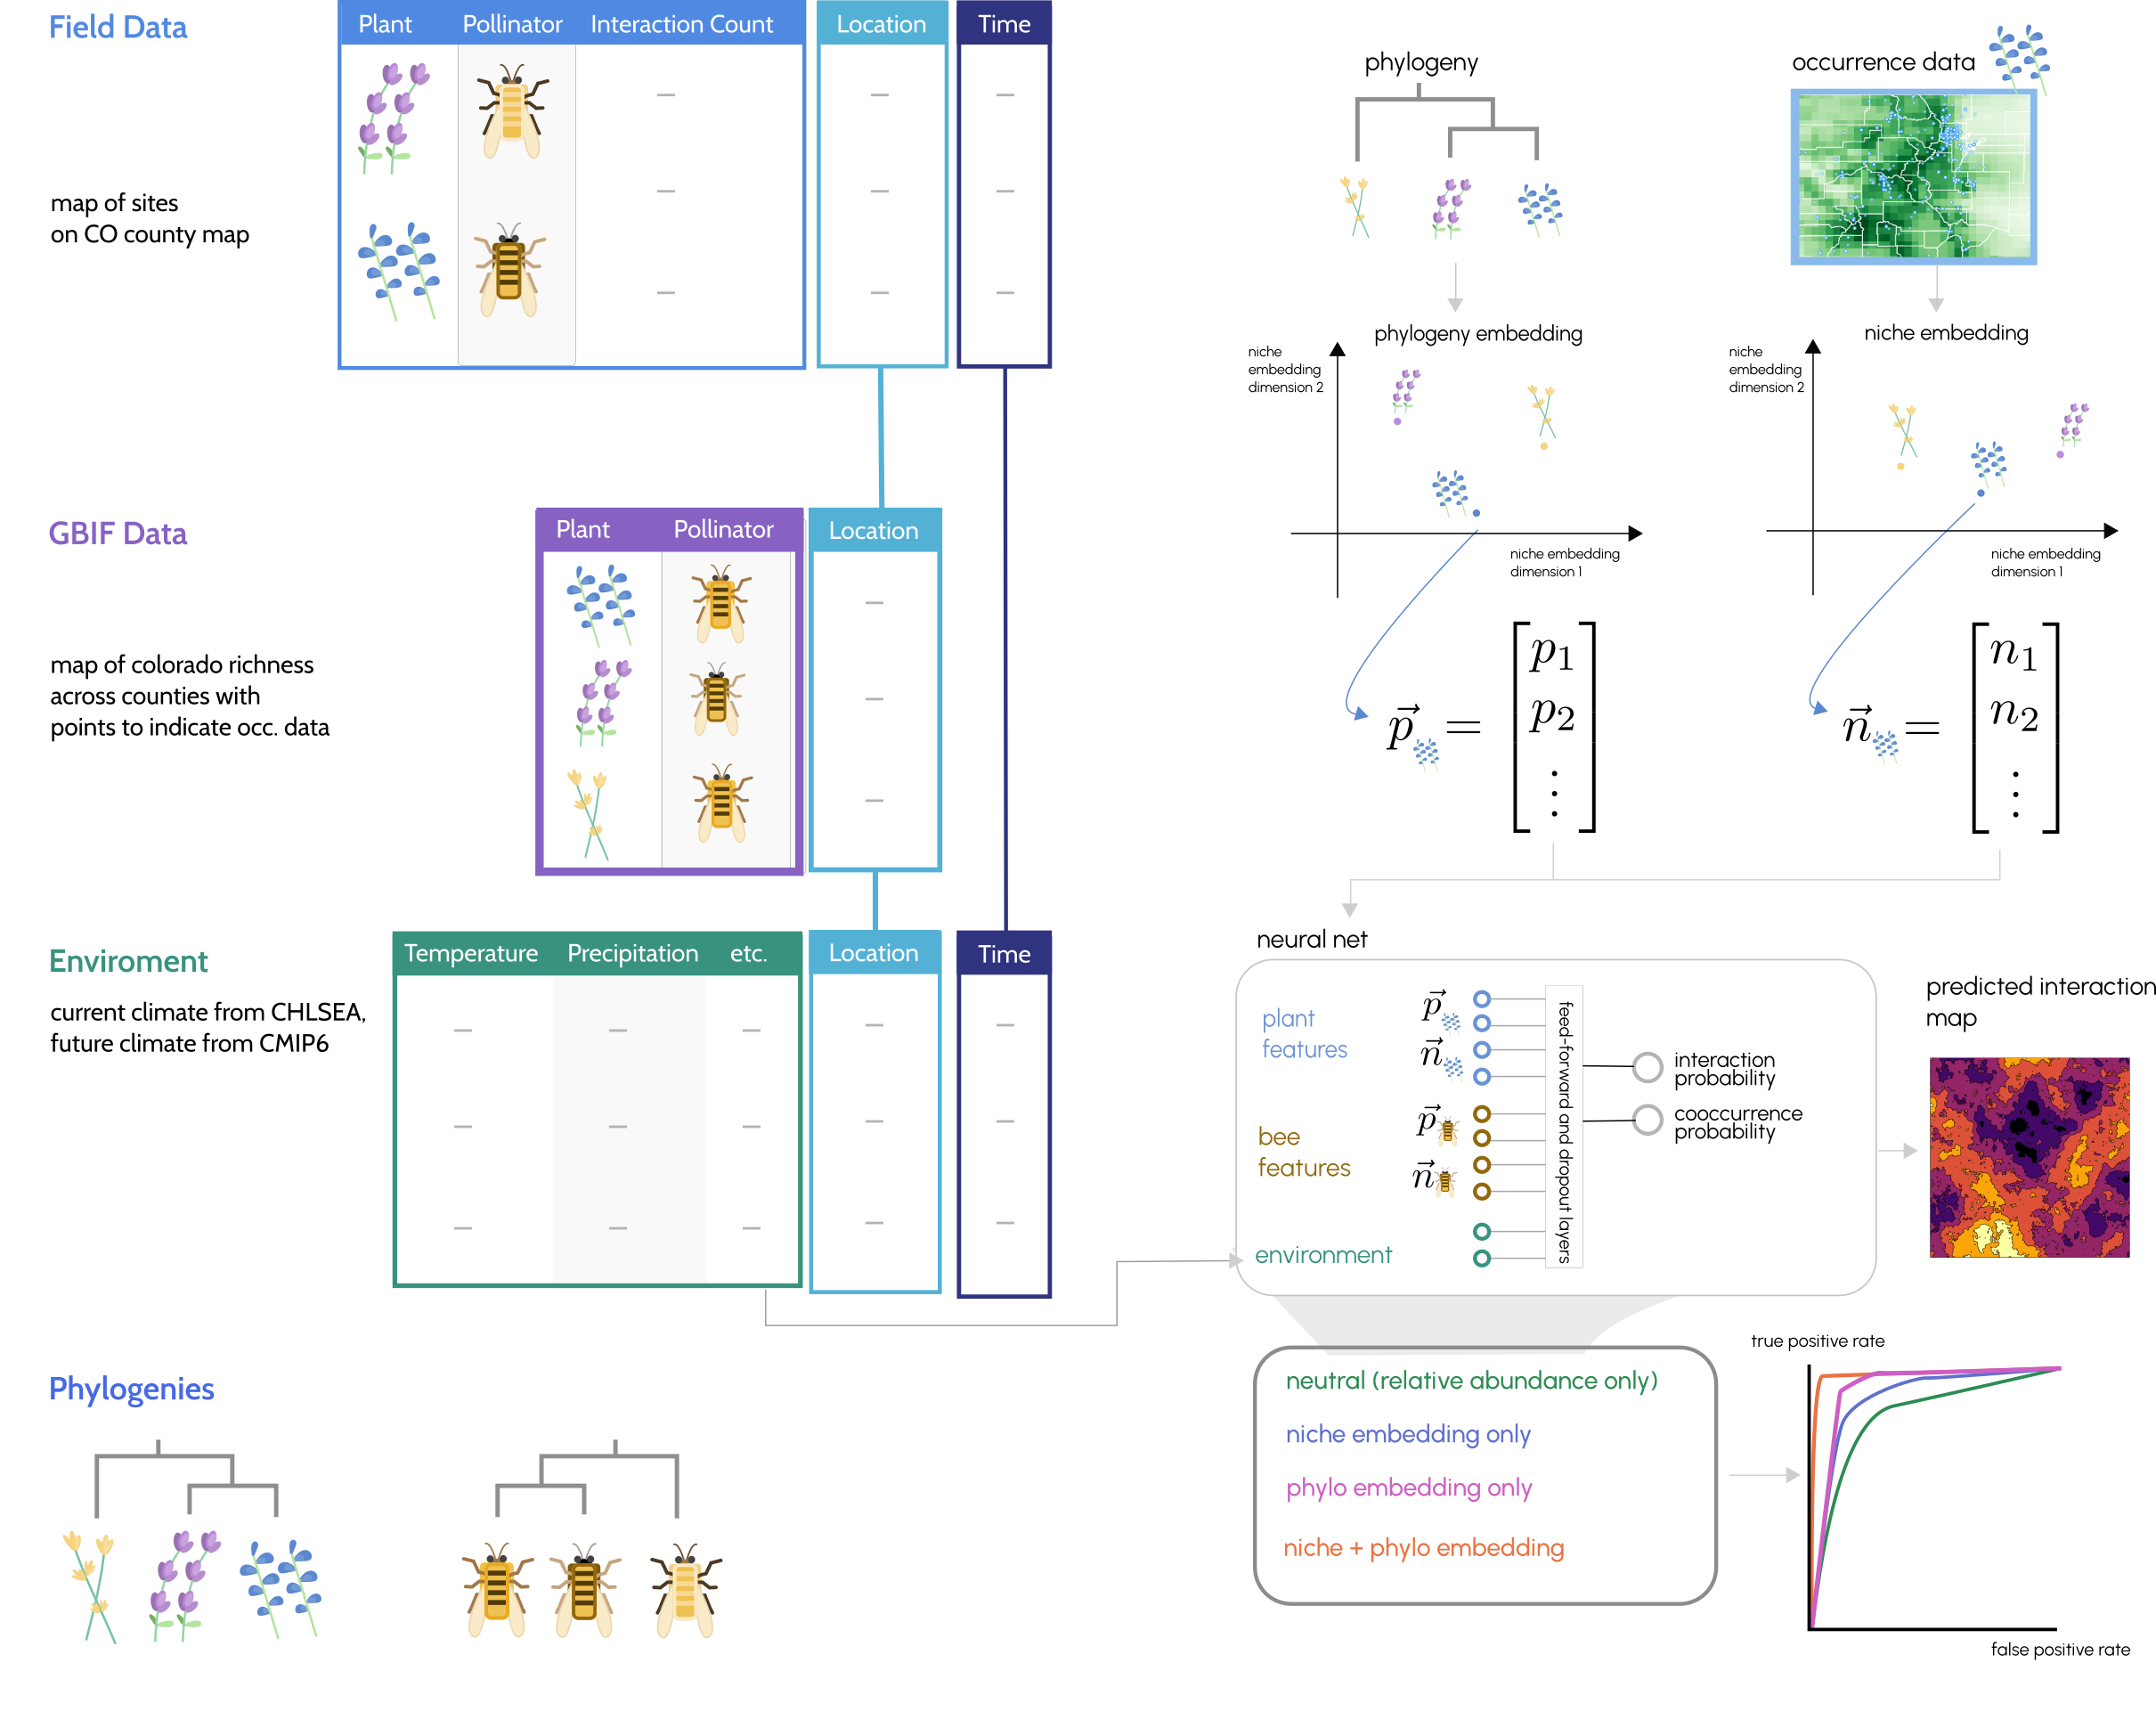
\includegraphics{./figures/concept_v2.png}
\caption{todo}\label{fig:concept}
}
\end{figure}

\hypertarget{data}{%
\subsection{Data}\label{data}}

This project involves assembly and integration of data from a variety of
(both structured and unstructured) sources. This data can be divided
into four categories: field data, GBIF data, remote-sensing data, and
phylogenetic data.

\hypertarget{field-data}{%
\subsubsection{Field data}\label{field-data}}

The field data consists of: (1) a seven year data-set from Rocky
Mountain Biological Laboratory, consisting of season-long interaction
and phenology data six plots along an elevation gradient. (2) a similar
six year data set from Elk Meadows, CO, and (3) a year across a large
elevation gradient at Pikes Peak.

Additional in-situ environmental sensors.

The partitioning of this data into training, test, and validation sets
if described in the \emph{Models} section.

\hypertarget{gbif-data}{%
\subsubsection{GBIF data}\label{gbif-data}}

The data from Global Biodiversity Information Facility (GBIF) itself
comes in two forms: (1) spatial records of bumblebee and flower records
(2) sparsely available records of the plants a bee was observed on (TODO
details from Julian).

\hypertarget{remote-sensing-data}{%
\subsubsection{Remote-sensing data}\label{remote-sensing-data}}

The remote-sensing data consists of 15-arcsecond elevation
data(\textbf{GMTED2020?}, cite), and daily 1km resolution precipitation
and temperature from CHELSA (Karger \emph{et al.} 2021).

\hypertarget{phylogenic-data}{%
\subsubsection{Phylogenic data}\label{phylogenic-data}}

The phylogenetic data consists of genomic barcodes available from NCBI
GenBank.

\hypertarget{a-spatiotemporally-explicit-predictive-metaweb-model}{%
\subsection{A spatiotemporally explicit predictive metaweb
model}\label{a-spatiotemporally-explicit-predictive-metaweb-model}}

What does it mean for it to be ``spatiotemporally explicit?'' Well the
formal definition of a metaweb is total species pool and

We denote the predicted probability of two species, \(i\) and \(j\),
interacting a \(p_{ij}\). The outcome is here is to build a model \(f\),
or rather a set of candidate models, that take \(i\) and \(j\) and
inputs, and which potentially combine this with .features

\[p_{ij} = f(i,j)\]

\hypertarget{candidate-models}{%
\subsubsection{Candidate models}\label{candidate-models}}

\textbf{\emph{True Neutral}}:
\(f(i,j) = \frac{1}{\sum_i \sum_j 1} = 1 / (P\cdot F)\)

\textbf{\emph{Relative-abundance (interaction neutral)}}:
\(f(i,j) = A_i A_j\) where \(A_x\) is the relative abundance of species
\(x\).

\textbf{\emph{Relative-abundance + environment-embedding}}:
\(f(i,j) = g(i,j, E_i, E_j)\)

\textbf{\emph{Relative-abundance + phylogeny-embedding}}: \$\$

\textbf{\emph{Relative-abundance + environment-embedding +
phylogeny-embedding}}

In gravel et al 2017
\[P(X_{iy}, X_{jy}, L_{ijy} | E_y) = P(X_{iy},X_{jy}P(L_{ijy} | X_{iy}, X_{jy}, E_y)\]
Then decompose probability of co-occurence as
\[P(X_{iy}, X_{jy}) = P(X_{iy})P(X_{jy})\]

\hypertarget{model-fitting-and-validation}{%
\subsection{Model fitting and
validation}\label{model-fitting-and-validation}}

Models are implemented and fitted in Julia v1.6, using Turing.jl
{[}cite{]}

\hypertarget{training-test-validation-split-scheme}{%
\subsubsection{Training-test-validation split
scheme}\label{training-test-validation-split-scheme}}

How do this? Do we remove sites entirely? Years entirely? Perhaps pikes
peak would be best as a validation set as its only one year anyway and
is a larger elevation gradient.

\hypertarget{results}{%
\section{Results}\label{results}}

After comparing different combinations of features/model structures and
finding the `best' performing model on validation data.

\hypertarget{figure-one-spatial-species-pool-and-network-prediction}{%
\subsection{Figure one: spatial species pool and network
prediction}\label{figure-one-spatial-species-pool-and-network-prediction}}

Figure that is two panels: a map of total species richness and a map of
network properties across Colorado. This model doesn't consider time,
only other predictors.

\hypertarget{figure-two-phenology}{%
\subsection{Figure two: Phenology}\label{figure-two-phenology}}

Same as figure one but consists of maps but at different times of the
year (e.g. March, June, August) and uses both an interaction-predictor
and distribution-predictor that incorporate time into predictions

\hypertarget{figure-three-climate}{%
\subsection{Figure three: Climate}\label{figure-three-climate}}

Much as climate change has shifted temperature gradients to get warmer
toward the poles, it has also moved temperature gradients up in
elevation.

We can get a CMIP6 forecast of temperature and precipitation, and then
predict how many observed interactions in the field data will no longer
have their composing species' distributions overlap. Decompose temporal
component of overlap from spatial component.

\hypertarget{discussion}{%
\section{Discussion}\label{discussion}}

This predictive model should not be used as definitive prediction:
instead it reveals gaps in our sampling (where we have little confidence
in predictions---see uncertainty figure). Iterative forecasting
(\textbf{Diteze?}): use this model to guide sampling in the future to
validate and update the model, etc.

\hypertarget{acknowledgements}{%
\subsection{Acknowledgements}\label{acknowledgements}}

\hypertarget{references}{%
\section*{References}\label{references}}
\addcontentsline{toc}{section}{References}

\hypertarget{refs}{}
\begin{CSLReferences}{1}{0}
\leavevmode\hypertarget{ref-Karger2017CliHig}{}%
Karger, D.N., Conrad, O., Böhner, J., Kawohl, T., Kreft, H., Soria-Auza,
R.W., \emph{et al.} (2017). Climatologies at high resolution for the
earth's land surface areas. \emph{Scientific Data}, 4, 170122.

\leavevmode\hypertarget{ref-Karger2021GloDai}{}%
Karger, D.N., Wilson, A.M., Mahony, C., Zimmermann, N.E. \& Jetz, W.
(2021). Global daily 1km land surface precipitation based on cloud
cover-informed downscaling. \emph{arXiv:2012.10108 {[}physics{]}}.

\leavevmode\hypertarget{ref-Olesen2011MisFor}{}%
Olesen, J.M., Bascompte, J., Dupont, Y.L., Elberling, H., Rasmussen, C.
\& Jordano, P. (2011). Missing and forbidden links in mutualistic
networks. \emph{Proceedings of the Royal Society B: Biological
Sciences}, 278, 725--732.

\end{CSLReferences}

\end{document}
